\section{Dữ liệu và tiền xử lý}

\subsection{Mô tả bộ dữ liệu}
Đề tài sử dụng bộ dữ liệu \textbf{Telco Customer Churn} do IBM công bố, được chia sẻ công khai trên Kaggle\footnote{\url{https://www.kaggle.com/datasets/blastchar/telco-customer-churn}}. Bộ dữ liệu gồm \textbf{7.043 khách hàng} và \textbf{21 cột}: một mã định danh \texttt{customerID}, 19 đặc trưng đầu vào và nhãn mục tiêu \texttt{Churn}.

\begin{table}[H]
\centering
\begin{tabular}{p{4cm} p{8.5cm} l}
\toprule
\textbf{Nhóm thông tin} & \textbf{Các cột} & \textbf{Kiểu} \\
\midrule
Nhân khẩu học & \texttt{gender}, \texttt{SeniorCitizen}, \texttt{Partner}, \texttt{Dependents} & Phân loại / nhị phân \\
Dịch vụ & \texttt{PhoneService}, \texttt{MultipleLines}, \texttt{InternetService}, \texttt{OnlineSecurity}, \texttt{OnlineBackup}, \texttt{DeviceProtection}, \texttt{TechSupport}, \texttt{StreamingTV}, \texttt{StreamingMovies} & Phân loại \\
Hợp đồng, thanh toán & \texttt{Contract}, \texttt{PaperlessBilling}, \texttt{PaymentMethod} & Phân loại \\
Chi phí & \texttt{MonthlyCharges}, \texttt{TotalCharges} & Số thực \\
Thời gian sử dụng & \texttt{tenure} (tháng) & Số nguyên \\
Nhãn & \texttt{Churn} (Yes/No) & Nhị phân \\
\bottomrule
\end{tabular}
\caption{Các nhóm thuộc tính trong bộ dữ liệu Telco Customer Churn}
\end{table}

\subsection{Kiểm tra chất lượng dữ liệu}
Quá trình khám phá dữ liệu được thực hiện trong notebook \texttt{01\_eda.ipynb} và được đóng gói lại thành hàm \texttt{load\_and\_clean\_data()} trong \texttt{src/data.py}. Các kết quả kiểm tra chính:
\begin{itemize}
    \item Không có dòng trùng lặp; \texttt{customerID} không thiếu và không trùng.
    \item Cột \texttt{TotalCharges} được đọc dưới dạng chuỗi và chứa \textbf{11 giá trị chỉ gồm khoảng trắng}. Các giá trị này được chuyển thành giá trị thiếu (NaN), sau đó cột được ép sang kiểu số. Ngoài 11 trường hợp này không có giá trị nào không thể chuyển thành số.
    \item Cả 11 khách hàng thiếu \texttt{TotalCharges} đều có \texttt{tenure} $= 0$, tức là khách hàng mới chưa phát sinh hóa đơn. Nhóm quyết định không thay cứng bằng 0 mà để bước \textit{imputation} trong pipeline xử lý.
    \item Không có giá trị âm. \texttt{tenure} nằm trong khoảng 0--72 tháng; \texttt{MonthlyCharges} trong khoảng 18{,}25--118{,}75; \texttt{TotalCharges} trong khoảng 18{,}80--8.684{,}80.
    \item Các giá trị \textit{``No internet service''} và \textit{``No phone service''} phản ánh tình trạng sử dụng dịch vụ, không phải giá trị thiếu, nên được giữ nguyên như một hạng mục riêng.
\end{itemize}

Hàm làm sạch kiểm tra chặt chẽ các điều kiện trên và báo lỗi nếu dữ liệu đầu vào không hợp lệ:

\begin{lstlisting}[style=pythonstyle, caption={Làm sạch TotalCharges và mã hóa nhãn trong \texttt{src/data.py}}]
for column in text_columns:
    df[column] = df[column].str.strip().replace("", float("nan"))

total_charges = pd.to_numeric(df["TotalCharges"], errors="coerce")
invalid_values = df["TotalCharges"].notna() & total_charges.isna()
if invalid_values.any():
    raise ValueError("TotalCharges contains non-numeric values")
df["TotalCharges"] = total_charges

df["Churn"] = df["Churn"].map({"No": 0, "Yes": 1})
\end{lstlisting}

\subsection{Phân bố nhãn và chia dữ liệu}
Trên toàn bộ dữ liệu có 5.174 khách hàng không rời bỏ (73{,}46\%) và 1.869 khách hàng rời bỏ (26{,}54\%). Dữ liệu \textbf{mất cân bằng ở mức vừa phải} (tỉ lệ xấp xỉ 2{,}8 : 1), vì vậy Accuracy không được dùng làm chỉ số duy nhất.

Dữ liệu được chia \textbf{Train/Test theo tỉ lệ 80/20} bằng \texttt{train\_test\_split} với \texttt{stratify=Churn} và \texttt{random\_state=42}:
\begin{itemize}
    \item Train: 5.634 khách hàng (tỉ lệ churn 26{,}54\%).
    \item Test: 1.409 khách hàng (tỉ lệ churn 26{,}54\%).
\end{itemize}
Danh sách \texttt{customerID} của mỗi tập được lưu vào \texttt{data/splits/train\_ids.csv} và \texttt{test\_ids.csv}. Mọi thực nghiệm sau đó đều đọc lại đúng hai danh sách này, đảm bảo \textbf{cùng một cách chia dữ liệu} cho mọi mô hình. Tập test được giữ riêng hoàn toàn, chỉ dùng cho đánh giá cuối cùng; mọi phân tích EDA chuyên sâu và lựa chọn mô hình đều thực hiện trên tập train.

\begin{figure}[H]
\centering
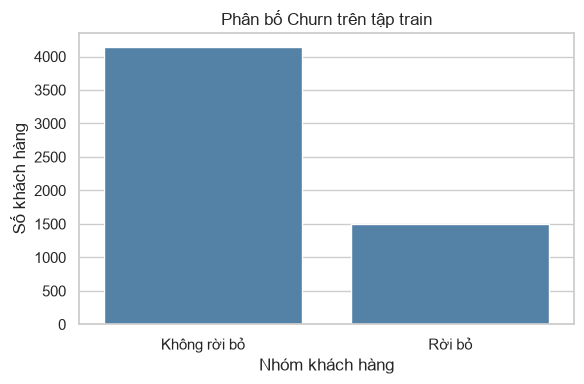
\includegraphics[width=0.5\textwidth]{img/eda_churn_distribution.png}
\caption{Phân bố nhãn Churn trên tập train}
\end{figure}

\subsection{Phân tích khám phá (EDA)}\label{sec:eda}

\subsubsection{Đặc trưng số}
\begin{figure}[H]
\centering
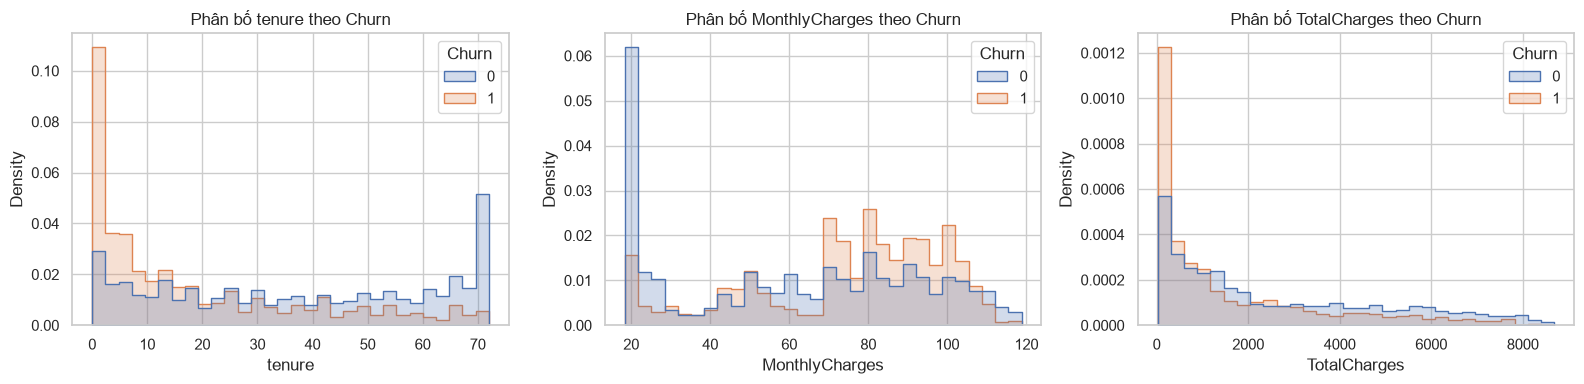
\includegraphics[width=\textwidth]{img/eda_numeric_hist.png}
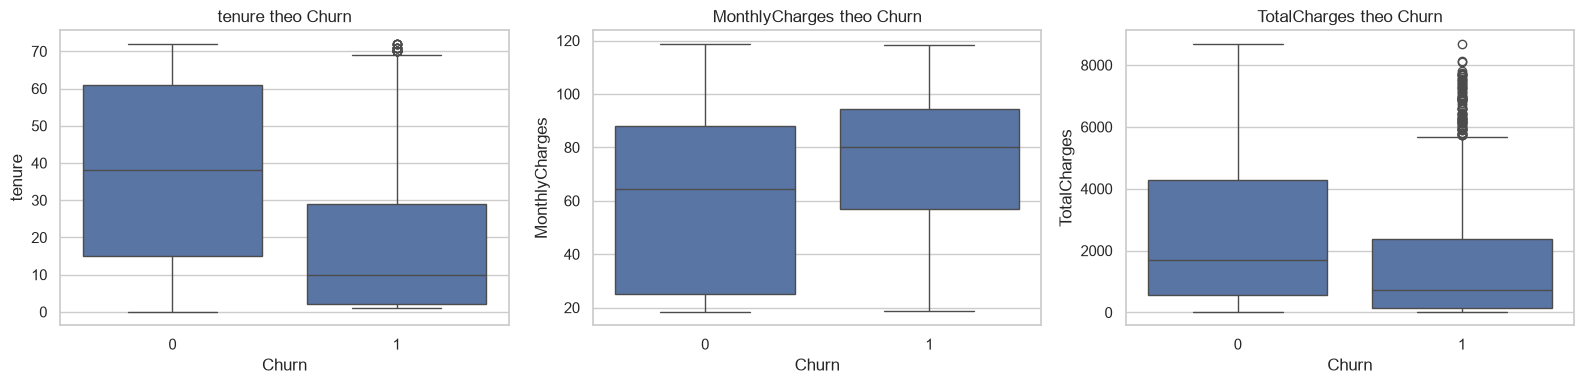
\includegraphics[width=\textwidth]{img/eda_numeric_boxplot.png}
\caption{Phân bố \texttt{tenure}, \texttt{MonthlyCharges}, \texttt{TotalCharges} theo Churn (tập train)}
\end{figure}

\begin{itemize}
    \item Khách hàng rời bỏ có xu hướng có \texttt{tenure} ngắn hơn rõ rệt; hệ số tương quan giữa \texttt{tenure} và Churn khoảng $-0{,}35$.
    \item Nhóm rời bỏ có \texttt{MonthlyCharges} nghiêng về mức cao (tương quan khoảng $+0{,}20$) và \texttt{TotalCharges} thấp hơn (tương quan khoảng $-0{,}19$).
    \item \texttt{tenure} và \texttt{TotalCharges} tương quan cao (khoảng $0{,}83$), \texttt{MonthlyCharges} và \texttt{TotalCharges} tương quan khoảng $0{,}65$. Điều này hợp lý vì tổng chi phí xấp xỉ bằng chi phí tháng nhân thời gian sử dụng.
    \item Một số điểm nằm ngoài râu boxplot nhưng đều nằm trong miền giá trị hợp lý, nên \textbf{không bị loại bỏ}.
\end{itemize}

\begin{figure}[H]
\centering
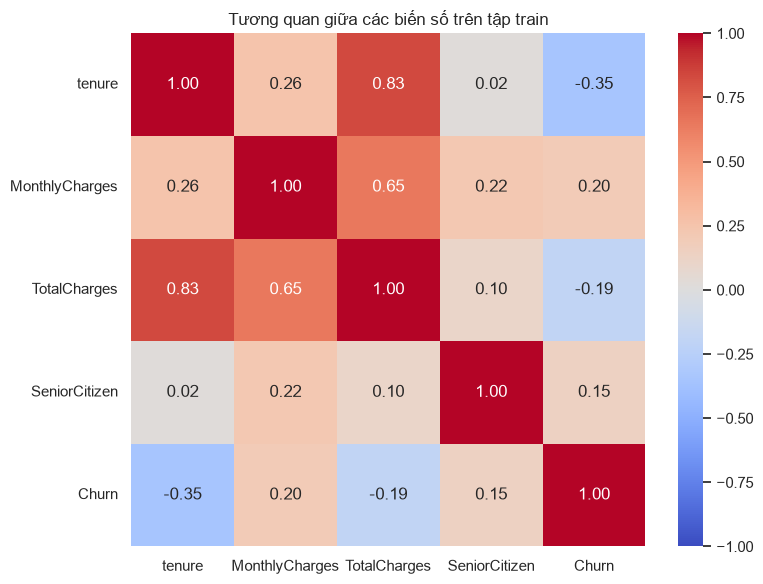
\includegraphics[width=0.55\textwidth]{img/eda_correlation.png}
\caption{Ma trận tương quan giữa các biến số và Churn trên tập train}
\end{figure}

\subsubsection{Đặc trưng phân loại}

\begin{table}[H]
\centering
\begin{tabular}{llrr}
\toprule
\textbf{Đặc trưng} & \textbf{Giá trị} & \textbf{Số khách hàng} & \textbf{Tỉ lệ churn} \\
\midrule
\multirow{3}{*}{Contract} & Month-to-month & 3.102 & \textbf{42,75\%} \\
 & One year & 1.173 & 11,08\% \\
 & Two year & 1.359 & 2,87\% \\
\midrule
\multirow{3}{*}{InternetService} & Fiber optic & 2.483 & \textbf{42,09\%} \\
 & DSL & 1.937 & 18,69\% \\
 & No & 1.214 & 7,25\% \\
\midrule
\multirow{4}{*}{PaymentMethod} & Electronic check & 1.891 & \textbf{45,74\%} \\
 & Mailed check & 1.286 & 19,28\% \\
 & Bank transfer (automatic) & 1.244 & 16,16\% \\
 & Credit card (automatic) & 1.213 & 14,92\% \\
\midrule
\multirow{2}{*}{TechSupport} & No & 2.771 & 41,75\% \\
 & Yes & 1.649 & 15,16\% \\
\midrule
\multirow{2}{*}{OnlineSecurity} & No & 2.797 & 41,94\% \\
 & Yes & 1.623 & 14,42\% \\
\midrule
\multirow{2}{*}{SeniorCitizen} & 1 & 920 & 41,09\% \\
 & 0 & 4.714 & 23,70\% \\
\bottomrule
\end{tabular}
\caption{Tỉ lệ churn theo một số đặc trưng phân loại (tập train)}
\end{table}

\begin{figure}[H]
\centering
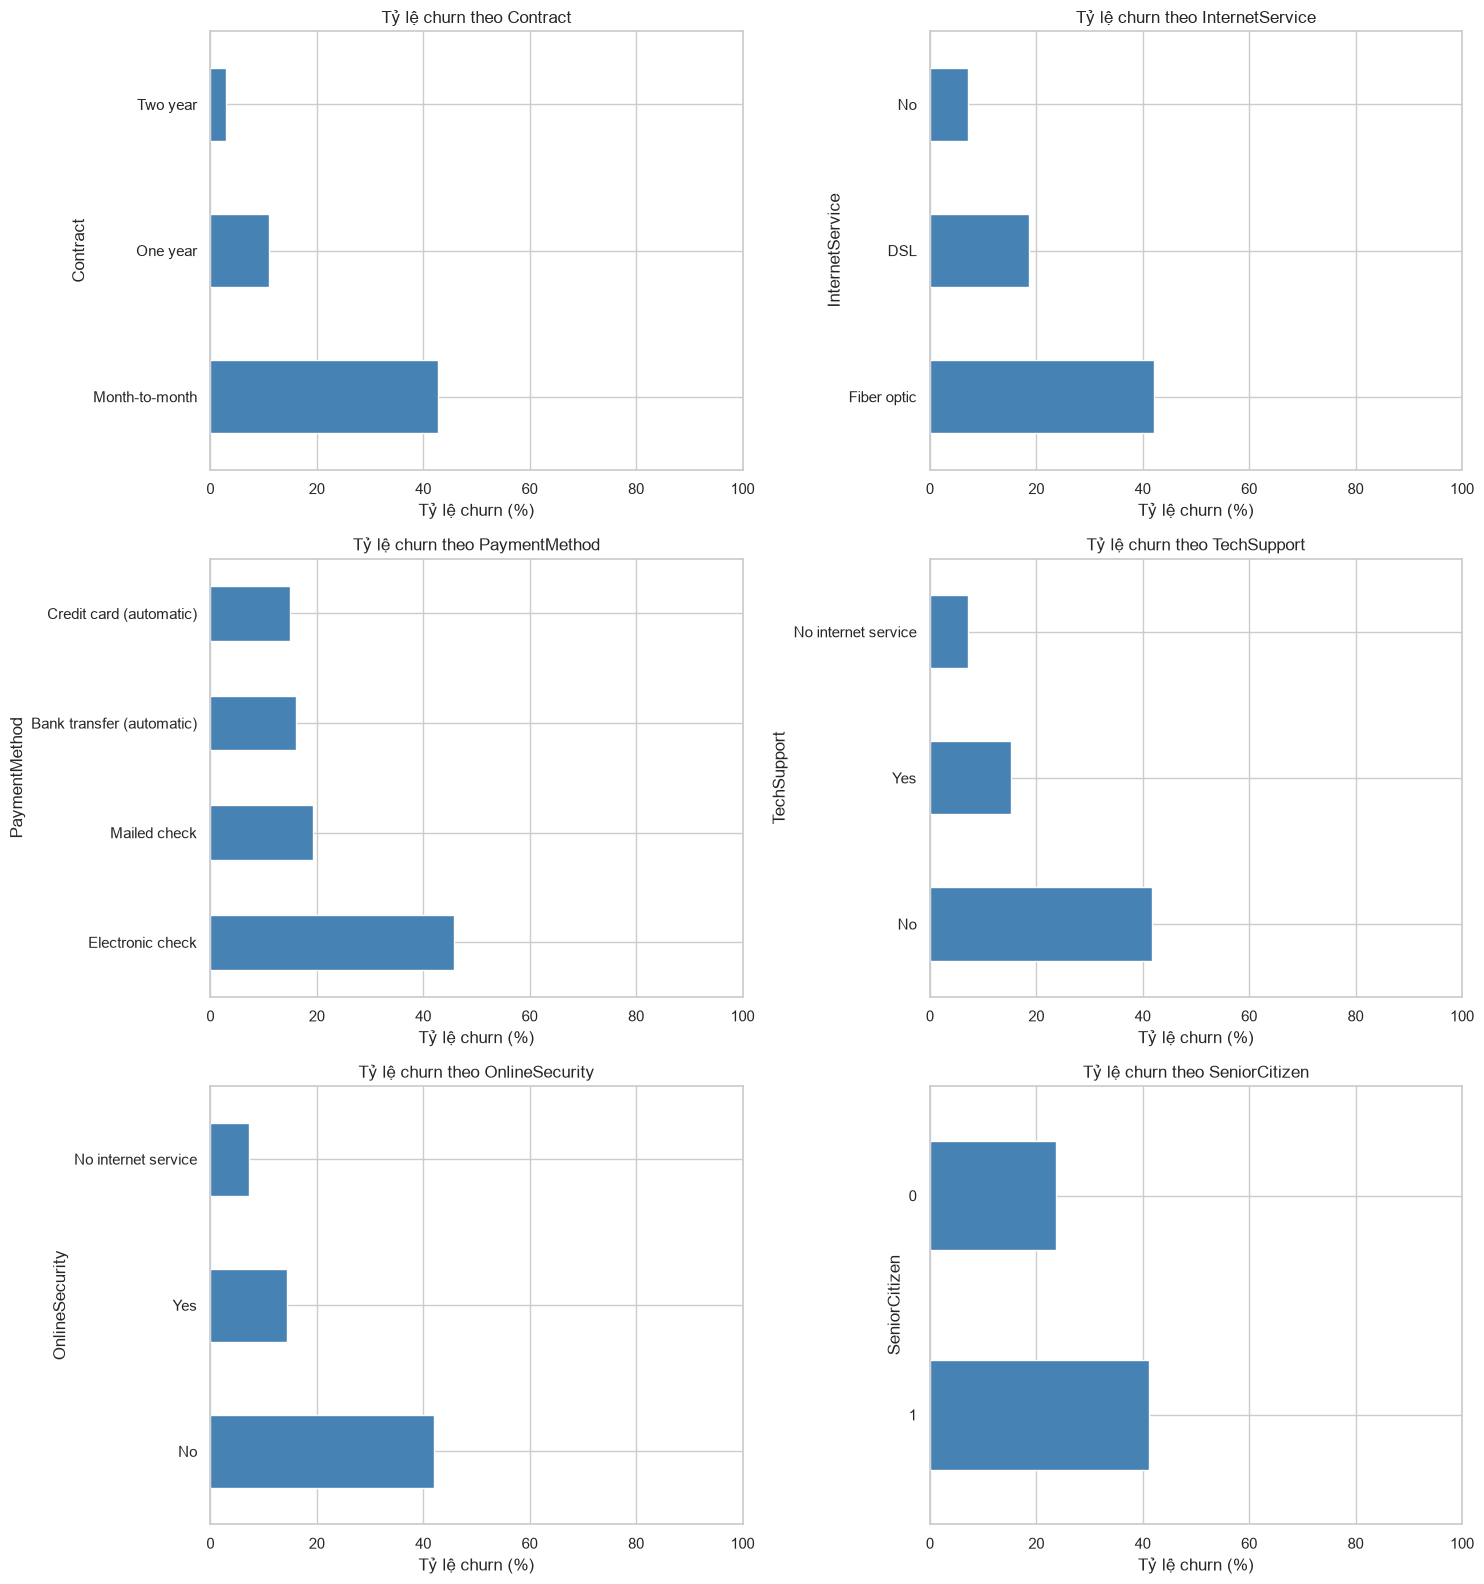
\includegraphics[width=0.85\textwidth]{img/eda_categorical_churn_rate.png}
\caption{Tỉ lệ churn theo các đặc trưng phân loại tiêu biểu}
\end{figure}

Nhận xét chính:
\begin{itemize}
    \item \textbf{Loại hợp đồng} là yếu tố phân tách mạnh nhất: hợp đồng theo tháng có tỉ lệ churn cao gấp gần 15 lần hợp đồng hai năm.
    \item Khách hàng dùng \textbf{Fiber optic}, thanh toán bằng \textbf{Electronic check}, \textbf{không} đăng ký TechSupport/OnlineSecurity hoặc là \textbf{người cao tuổi} có tỉ lệ churn cao hơn hẳn.
    \item Đây là các mối liên hệ quan sát được từ dữ liệu, chưa chứng minh quan hệ nhân quả và chưa xét tương tác giữa các yếu tố (ví dụ Fiber optic thường đi kèm mức phí cao).
\end{itemize}

\subsection{Pipeline tiền xử lý}
Từ kết quả EDA, nhóm xây dựng bộ tiền xử lý bằng \texttt{ColumnTransformer} của \texttt{scikit-learn} (\texttt{src/preprocessing.py}). Đặc trưng được chia thành ba nhóm:

\begin{table}[H]
\centering
\begin{tabular}{p{3.2cm} p{5.5cm} p{6.5cm}}
\toprule
\textbf{Nhóm} & \textbf{Cột} & \textbf{Biến đổi} \\
\midrule
Số (3) & \texttt{tenure}, \texttt{MonthlyCharges}, \texttt{TotalCharges} & \texttt{SimpleImputer(median)} $\rightarrow$ \texttt{StandardScaler} (chỉ với Logistic Regression) \\
Nhị phân (1) & \texttt{SeniorCitizen} & Giữ nguyên mã 0/1 (\texttt{passthrough}) \\
Phân loại (15) & Các cột còn lại & \texttt{SimpleImputer(most\_frequent)} $\rightarrow$ \texttt{OneHotEncoder(handle\_unknown="ignore")} \\
\bottomrule
\end{tabular}
\caption{Các bước tiền xử lý theo nhóm đặc trưng}
\end{table}

\begin{lstlisting}[style=pythonstyle, caption={Hàm xây dựng bộ tiền xử lý trong \texttt{src/preprocessing.py}}]
def build_preprocessor(scale_numeric: bool = True) -> ColumnTransformer:
    numeric_steps = [("imputer", SimpleImputer(strategy="median"))]
    if scale_numeric:
        numeric_steps.append(("scaler", StandardScaler()))

    categorical_pipeline = Pipeline(steps=[
        ("imputer", SimpleImputer(strategy="most_frequent")),
        ("encoder", OneHotEncoder(handle_unknown="ignore",
                                  sparse_output=False)),
    ])
    return ColumnTransformer(
        transformers=[
            ("numeric", Pipeline(numeric_steps), NUMERIC_FEATURES),
            ("binary", "passthrough", BINARY_FEATURES),
            ("categorical", categorical_pipeline, CATEGORICAL_FEATURES),
        ],
        remainder="drop",
    )
\end{lstlisting}

Các quyết định thiết kế:
\begin{itemize}
    \item \texttt{customerID} được giữ lại để truy vết và tái tạo cách chia dữ liệu nhưng bị loại khỏi đầu vào mô hình (\texttt{remainder="drop"}).
    \item Sau One-Hot Encoding, 19 đặc trưng gốc trở thành vector khoảng 45 chiều.
    \item \texttt{handle\_unknown="ignore"} giúp pipeline không bị lỗi khi dự đoán khách hàng mới có giá trị phân loại chưa từng gặp (được kiểm thử trực tiếp trong \texttt{preprocessing.py}).
    \item \texttt{StandardScaler} chỉ được bật cho Logistic Regression (hàm \texttt{requires\_scaling()}), vì các mô hình cây không phụ thuộc vào thang đo.
    \item Bộ tiền xử lý và mô hình được ghép trong một \texttt{Pipeline} duy nhất. Khi cross-validation, imputer/scaler/encoder chỉ được \texttt{fit} trên phần huấn luyện của từng fold, tránh \textbf{rò rỉ dữ liệu} (\textit{data leakage}) từ fold validation.
\end{itemize}

\subsection{Feature Engineering}
Dựa trên các quan sát từ EDA, nhóm xây dựng 9 đặc trưng mới trong transformer \texttt{ChurnFeatureEngineer} (\texttt{src/features.py}):

\begin{table}[H]
\centering
\begin{tabular}{l l p{8.3cm}}
\toprule
\textbf{Loại} & \textbf{Đặc trưng} & \textbf{Cách tính và lý do} \\
\midrule
\multirow{3}{*}{Số} & \texttt{num\_services} & Số dịch vụ khách hàng đăng ký: số cột có giá trị ``Yes'' trong 8 cột dịch vụ, cộng 1 nếu có dùng Internet. Khách dùng nhiều dịch vụ được kỳ vọng gắn bó hơn. \\
 & \texttt{avg\_monthly\_charge} & \texttt{TotalCharges / tenure}; khách có \texttt{tenure} $=0$ (chưa có \texttt{TotalCharges}) lấy \texttt{MonthlyCharges}. \\
 & \texttt{charge\_diff} & \texttt{MonthlyCharges} $-$ \texttt{avg\_monthly\_charge}; dương nghĩa là phí hiện tại cao hơn mức trung bình đã trả (vừa tăng giá hoặc nâng gói). \\
\midrule
\multirow{3}{*}{Nhị phân} & \texttt{is\_new\_month\_to\_month} & 1 nếu hợp đồng theo tháng \textit{và} \texttt{tenure} $\le 12$ -- nhóm rủi ro cao nhất theo EDA. \\
 & \texttt{fiber\_no\_tech\_support} & 1 nếu dùng Fiber optic nhưng không đăng ký TechSupport. \\
 & \texttt{is\_auto\_payment} & 1 nếu thanh toán tự động (chuyển khoản hoặc thẻ tín dụng). \\
\midrule
\multirow{3}{*}{Phân loại} & \texttt{tenure\_group} & Rời rạc hóa \texttt{tenure} thành 0--12, 13--24, 25--48, 49+ tháng. \\
 & \texttt{monthly\_charge\_group} & Chia \texttt{MonthlyCharges} thành 4 nhóm theo tứ phân vị (Q1--Q4). \\
 & \texttt{contract\_tenure} & Kết hợp Contract và \texttt{tenure\_group}, ví dụ ``Month-to-month\_0-12''. \\
\bottomrule
\end{tabular}
\caption{Các đặc trưng mới trong Feature Engineering}
\end{table}

Thiết kế cài đặt:
\begin{itemize}
    \item \texttt{ChurnFeatureEngineer} là một transformer theo chuẩn \texttt{scikit-learn} (\texttt{BaseEstimator}, \texttt{TransformerMixin}), được đặt làm bước đầu tiên của \texttt{Pipeline}, trước \texttt{ColumnTransformer}. Nhờ vậy các đặc trưng được tạo nhất quán cho train, validation, test và khách hàng mới trong \texttt{predict.py}.
    \item Ngưỡng chia nhóm \texttt{MonthlyCharges} là tứ phân vị \textbf{học từ dữ liệu} trong hàm \texttt{fit}. Vì transformer nằm trong Pipeline, các ngưỡng này chỉ được tính trên phần huấn luyện của mỗi fold, không rò rỉ thông tin từ fold validation. Ngưỡng ngoài cùng được đặt là $\pm\infty$ để mọi giá trị mới đều thuộc một nhóm.
    \item Đặc trưng số mới đi qua nhánh imputer/scaler, đặc trưng nhị phân giữ nguyên, đặc trưng phân loại mới đi qua nhánh One-Hot Encoding. Sau FE, dữ liệu có 28 cột trước khi mã hóa.
    \item Bật bằng tham số dòng lệnh \texttt{--feature-engineering} của \texttt{train.py} và \texttt{tune.py}.
\end{itemize}

\begin{lstlisting}[style=pythonstyle, caption={Một phần \texttt{ChurnFeatureEngineer} trong \texttt{src/features.py}}]
def fit(self, X, y=None):
    # Nguong nhom MonthlyCharges hoc tu fold train (tu phan vi).
    quantiles = np.linspace(0, 1, self.n_charge_bins + 1)
    edges = np.quantile(X["MonthlyCharges"], quantiles)
    edges[0], edges[-1] = -np.inf, np.inf
    self.charge_edges_ = np.unique(edges)
    return self

def transform(self, X):
    X = X.copy()
    tenure = X["tenure"]
    X["avg_monthly_charge"] = np.where(
        tenure > 0, X["TotalCharges"] / tenure.where(tenure > 0),
        X["MonthlyCharges"])
    X["charge_diff"] = X["MonthlyCharges"] - X["avg_monthly_charge"]
    X["is_new_month_to_month"] = (
        X["Contract"].eq("Month-to-month") & (tenure <= 12)).astype(int)
    ...
\end{lstlisting}
